\documentclass[11pt]{article}
\usepackage[final]{acl}   % EMNLP 2026 demo = single-blind (authors shown). Switch to [review] if needed.
\usepackage{times}
\usepackage{latexsym}
\usepackage[T1]{fontenc}
\usepackage[utf8]{inputenc}
\usepackage{microtype}
\usepackage{graphicx}
\usepackage{subcaption}
\usepackage{booktabs}
\usepackage{enumitem}
\usepackage{amssymb}
\usepackage{xcolor}
\usepackage{url}

\captionsetup[sub]{font=small,skip=2pt}

\newcommand{\yes}{\textcolor{green!55!black}{\checkmark}}
\newcommand{\pmark}{\textcolor{orange!85!black}{$\sim$}}
\newcommand{\no}{\textcolor{red!70!black}{$\times$}}

\title{PolyInterview: A Deployed Multi-Agent System for Immersive,\\ Explainable, and Multimodal Mock-Interview Practice}

% Single-blind, non-anonymous. TODO(authors): confirm exact emails for co-authors before submission.
\author{
  \normalfont Zhiyuan Wen$^{1}$, Jiannong Cao$^{1}$, Zijian Wang$^{1}$, Chen Chen$^{1}$, \\
  \normalfont Xiaoyun Liu$^{1}$, Jianing Yin$^{1}$, Zhuo Li$^{2}$ \\[3pt]
  \normalfont $^{1}$Department of Computing, The Hong Kong Polytechnic University, Hong Kong, China \\
  \normalfont $^{2}$School of Artificial Intelligence, Chongqing University of Posts and Telecommunications, China \\[3pt]
  \normalfont\texttt{\{zyuanwen, jiannong.cao, zi-jian.wang\}@polyu.edu.hk} \\
  \normalfont\texttt{\{chen03.chen, xiaoyun.liu, jianing-laetitia.yin\}@connect.polyu.hk} \\
  \normalfont\texttt{cliff.zhuo.li@gmail.com}
}

\begin{document}
\maketitle

\begin{abstract}
Interview practice is scarce and expensive, and the feedback that decides a real hiring outcome (how you reason, how you speak, how you carry yourself) is exactly what solo practice cannot give back. Existing AI interview tools tailor only the first question, walk a fixed list without follow-ups, narrow their scoring to the transcript, and rarely tie a number to a reason. We present \textbf{PolyInterview}, a publicly deployed multi-agent system in which a student rehearses a complete, embodied mock interview with a lip-synced digital-human interviewer that adapts its follow-ups, and then receives feedback that is multi-dimensional and \emph{traceable}. A planner agent assembles a personalized question list from the job description and CV; an interviewer agent decides follow-ups from a live check of each answer's consistency, clarity, and relevance; and four feature agents run in parallel over text, audio, and video, producing thirteen behavioral features that a three-layer architecture rolls up into ten competency aspects and two proficiency tracks, grounded in the established KSA and STAR hiring frameworks. The paper is built around the running system: we walk through the six screens a student actually touches, from a two-panel live interview to a report where every score expands into the behavioral signal beneath it. PolyInterview is deployed and live,\footnote{Live demo: \url{https://polyinterview.comp.polyu.edu.hk/}. Screencast ($\leq$2.5\,min, MPEG4) submitted separately.} has reached students across six institutions in a two-round pilot, and ships with a $\leq$2.5-minute screencast walking through one end-to-end session. Reanalyzing a cleaned 120-session deployment corpus, we find that the per-feature architecture does something benchmarks hide: it makes its own failure modes legible. Most sharply, the non-verbal evaluator silently returns a zero on 31.8\% of the answers it should have scored (74 of 233 video-relevant answers), which we report as both a finding and an agenda for validation.
\end{abstract}

\section{Introduction}
Hiring has tightened and shifted toward skills-based selection that probes both soft and hard skills \emph{inside} the interview. Good practice has not kept up. Real interviews are too rare to learn from, and expert mock coaching is costly and does not scale during peak recruiting. Practicing alone is worse than it looks: it never produces the probing follow-up that exposes a thin answer, and it gives no feedback on the voice and body language that interviewers read within the first minute. The cost is real: structured interviews predict job performance with a validity near $0.51$ \citep{schmidt1998validity}, and impressions formed from a few seconds of behavior already track the final decision \citep{ambady1992thin}. A candidate who cannot rehearse those signals is rehearsing the wrong thing.

AI is the natural response, and several products exist, but they share three gaps. \textbf{Personalization} stops early: question banks are generic, or only the opening question is tailored, with no reasoning over what the candidate just said. \textbf{Interaction} is shallow: a session advances through a fixed list whether an answer is sharp, vague, or self-contradictory, losing the multi-turn pressure of a real interview. \textbf{Assessment} is narrow and opaque: methods read the transcript and drop voice and non-verbal behavior, and even when a rubric is applied, its dimensions seldom map to any theory, so a score arrives without a reason a student can act on. The history here is cautionary: HireVue withdrew its facial-analysis feature in 2020 after sustained criticism. That makes \emph{explainable, advisory} non-verbal feedback the responsible target, not a reason to abandon the modality.

We organize the design around a frame from selection psychology: an offer is \textsc{Match} $\times$ \textsc{Convince}. \textsc{Match} is whether ability fits the role: the Knowledge, Skills, and Abilities (KSA) a recruiter looks for. \textsc{Convince} is whether the candidate communicates that fit. Because an offer is a product and not a sum, a useful system has to serve both sides in one loop. \textbf{PolyInterview} does so as a deployed, live system; to our knowledge it is among the first self-serve mock-interview tools to put a digital-human interviewer and a theory-grounded, multimodal, explainable evaluation pipeline in a single end-to-end interaction, and the axis it owns outright is per-feature traceable explanations bound to KSA$\times$STAR. Our contributions:
\begin{enumerate}[noitemsep,topsep=2pt,leftmargin=*]
  \item A working, publicly available mock-interview \emph{system} with an embodied digital-human interviewer and complete, multi-stage interviews rather than one-off Q\&A, presented here through the six screens a student actually uses (\S\ref{sec:system}).
  \item A multi-agent design in which a planner agent personalizes the question list and an interviewer agent generates follow-ups from a real-time answer check, extending personalization \emph{past} the first question with configurable difficulty (\S\ref{sec:match}).
  \item A three-layer, KSA$\times$STAR-grounded scoring pipeline with four parallel feature agents over text, audio, and video (13 features $\rightarrow$ 10 aspects $\rightarrow$ 2 tracks), where every score traces back to a behavioral signal and is surfaced that way in the report interface (\S\ref{sec:scoring}).
  \item A real deployment and a reanalysis of a cleaned 120-session corpus that turns the architecture's traceability into a concrete, actionable finding about evaluator reliability, plus a validation plan (\S\ref{sec:deploy}--\S\ref{sec:eval}).
\end{enumerate}

\section{Related Work}
\label{sec:related}

\begin{table*}[t]
\centering\small
\setlength{\tabcolsep}{4pt}
\begin{tabular}{lccccc}
\toprule
& \textbf{Adaptive} & \textbf{Theory-grounded} & \textbf{Multimodal} & \textbf{Multi-stage} & \textbf{Explainable} \\
& \textbf{follow-ups} & \textbf{feedback} & \textbf{(text/audio/video)} & \textbf{interview} & \textbf{\& traceable} \\
\midrule
\multicolumn{6}{l}{\emph{Commercial tools}} \\
Google Interview Warmup & \no & \pmark & \pmark & \no & \no \\
Yoodli & \no & \pmark & \pmark & \no & \no \\
Big Interview & \pmark & \pmark & \no & \no & \no \\
Final Round AI & \pmark & \pmark & \pmark & \no & \pmark \\
HireVue & \pmark & \pmark & \no\,(removed 2020) & \pmark & \no \\
Interviewing.io (human) & \yes & \yes & --- & \yes & \pmark \\
\midrule
\multicolumn{6}{l}{\emph{Research systems}} \\
MACH \citep{hoque2013mach} & \no & \no & \yes & \no & \yes \\
TARDIS \citep{anderson2013tardis} & \no & \no & \pmark & \pmark & \pmark \\
VR-JIT \citep{smith2014virtual} & \pmark & \pmark & \no & \pmark & \yes \\
ERICA interviewer \citep{inoue2020jobinterviewer} & \yes & \no & \no & \no & \no \\
EZInterviewer \citep{li2023ezinterviewer} & \pmark & \no & \no & \no & \no \\
MockLLM \citep{sun2025mockllm} & \yes & \no & \no & \no & \no \\
Conversate \citep{daryanto2025conversate} & \yes & \pmark & \no & \no & \yes \\
\midrule
\textbf{PolyInterview (ours)} & \yes & \yes\,(KSA$\times$STAR) & \yes & \yes & \yes \\
\bottomrule
\end{tabular}
\caption{Positioning against representative interview-practice tools and research systems. Commercial rows reflect public product information as of 2026; research rows reflect what each cited paper reports. \yes\ full, \pmark\ partial, \no\ absent.}
\label{tab:compare}
\end{table*}

\paragraph{Commercial AI interview tools.} Google Interview Warmup, Yoodli, Big Interview, HireVue, and Interviewing.io cover much of the practical market, and an LLM-era wave typified by Final Round AI layers resume-tailored mock sessions and per-question feedback on top of real-time interview copilots. Each solves part of the problem (delivery metrics, model answers, or human coaching), but as Table~\ref{tab:compare} lays out, none combines adaptive questioning, multimodal \emph{explainable} scoring, and a coherent multi-stage interview in one self-serve tool.

\paragraph{Virtual agents for interview training.} A pre-LLM line of HCI research already put an embodied agent in the interviewer's chair. MACH \citep{hoque2013mach} pairs a virtual coach with video-aligned feedback on smiles, prosody, and filler words; the TARDIS/Gloria line \citep{anderson2013tardis,baur2013job,langer2016dear} senses social cues in real time but follows a predetermined scenario without understanding the trainee's answers; VR-JIT \citep{smith2014virtual} gives RCT-validated, content-level explanations, but over pre-scripted response options rather than free speech. Later, ERICA \citep{inoue2020jobinterviewer} showed an android interviewer generating follow-ups from answer quality, yet returns no feedback at all. Across this line a system offers multimodal delivery sensing \emph{or} explainable content feedback, never both, and none can probe a free-form answer.

\paragraph{LLM-based mock interviews.} LLMs put answer-aware questioning back within reach. EZInterviewer \citep{li2023ezinterviewer} learns to generate mock-interview questions from real recruitment dialogs but offers no assessment; InterviewBot \citep{wang2023interviewbot} conducts deployed college-admission interviews end-to-end, again without feedback; MockLLM \citep{sun2025mockllm} simulates both sides of an interview for person--job matching rather than coaching; SimInterview \citep{nguyen2025siminterview} adds a talking-head interviewer and a multilingual voice pipeline; Conversate \citep{daryanto2025conversate} comes closest to our practice loop, pairing adaptive follow-ups with dialogic feedback anchored in the transcript. When these systems assess at all, they assess from text alone, with no theory-grounded rubric and no audio or video evidence: exactly the gap Table~\ref{tab:compare} makes visible.

\paragraph{Automated video interviews.} Work in affective computing and industrial-organizational psychology predicts interview constructs from multimodal features \citep{naim2018automated,hemamou2019hirenet}, usually by extracting hand-engineered signals and regressing them onto recruiter ratings. These pipelines can be accurate, but they emit a score, not the evidence behind it, which limits their use as a \emph{learning} tool and complicates accountability; their reliability and validity are also uneven across constructs \citep{hickman2022automated}. We instead frame video evaluation as an evidence-based, explainable process rather than score regression, and ship that stance in a deployed, student-facing system.

\paragraph{Foundation models as evaluators.} Using language and vision-language models as judges is now common \citep{zheng2023judging} and carries known biases. We use such models not as black-box raters but as agents in a layered pipeline whose intermediate features and aspects are exposed to the user and bound to established hiring frameworks, so a judgment can be inspected and argued with.

\section{System Overview}
\label{sec:system}

\begin{figure*}[t]
  \centering
  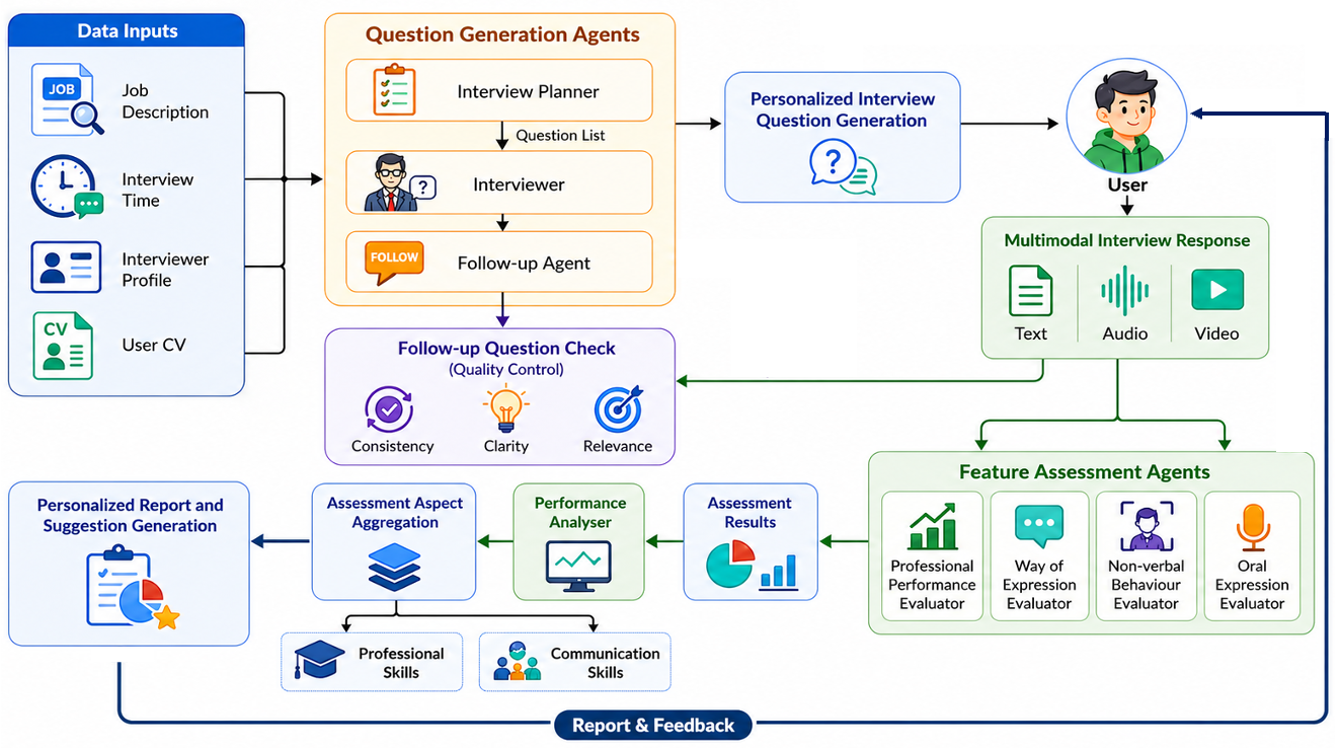
\includegraphics[width=0.9\textwidth]{figures/pipeline.png}
  \caption{The PolyInterview multi-agent architecture. Two questioning agents (Interview Planner and Interviewer) build a personalized session from the job description, interview time, interviewer profile, and CV; a Follow-up Question Check on each answer (consistency, clarity, relevance) gates further probing. The candidate's multimodal response (text, audio, video) is scored by four parallel feature-assessment agents, aggregated into two competency tracks, and turned into a personalized report and suggestions.}
  \label{fig:pipeline}
\end{figure*}

A session moves through four stages (Figure~\ref{fig:pipeline}): \emph{setup}, \emph{live interview}, \emph{evaluation}, and \emph{report}, driven by a multi-agent backend and a digital-human engine. From the student's side it is a short loop they can run at the live demo: configure one session, talk to the avatar, and read the report. Figure~\ref{fig:journey} shows that loop as the student sees it, and we use it to structure this section.

\begin{figure*}[t]
  \centering
  \begin{subfigure}[t]{0.485\textwidth}
    \centering
    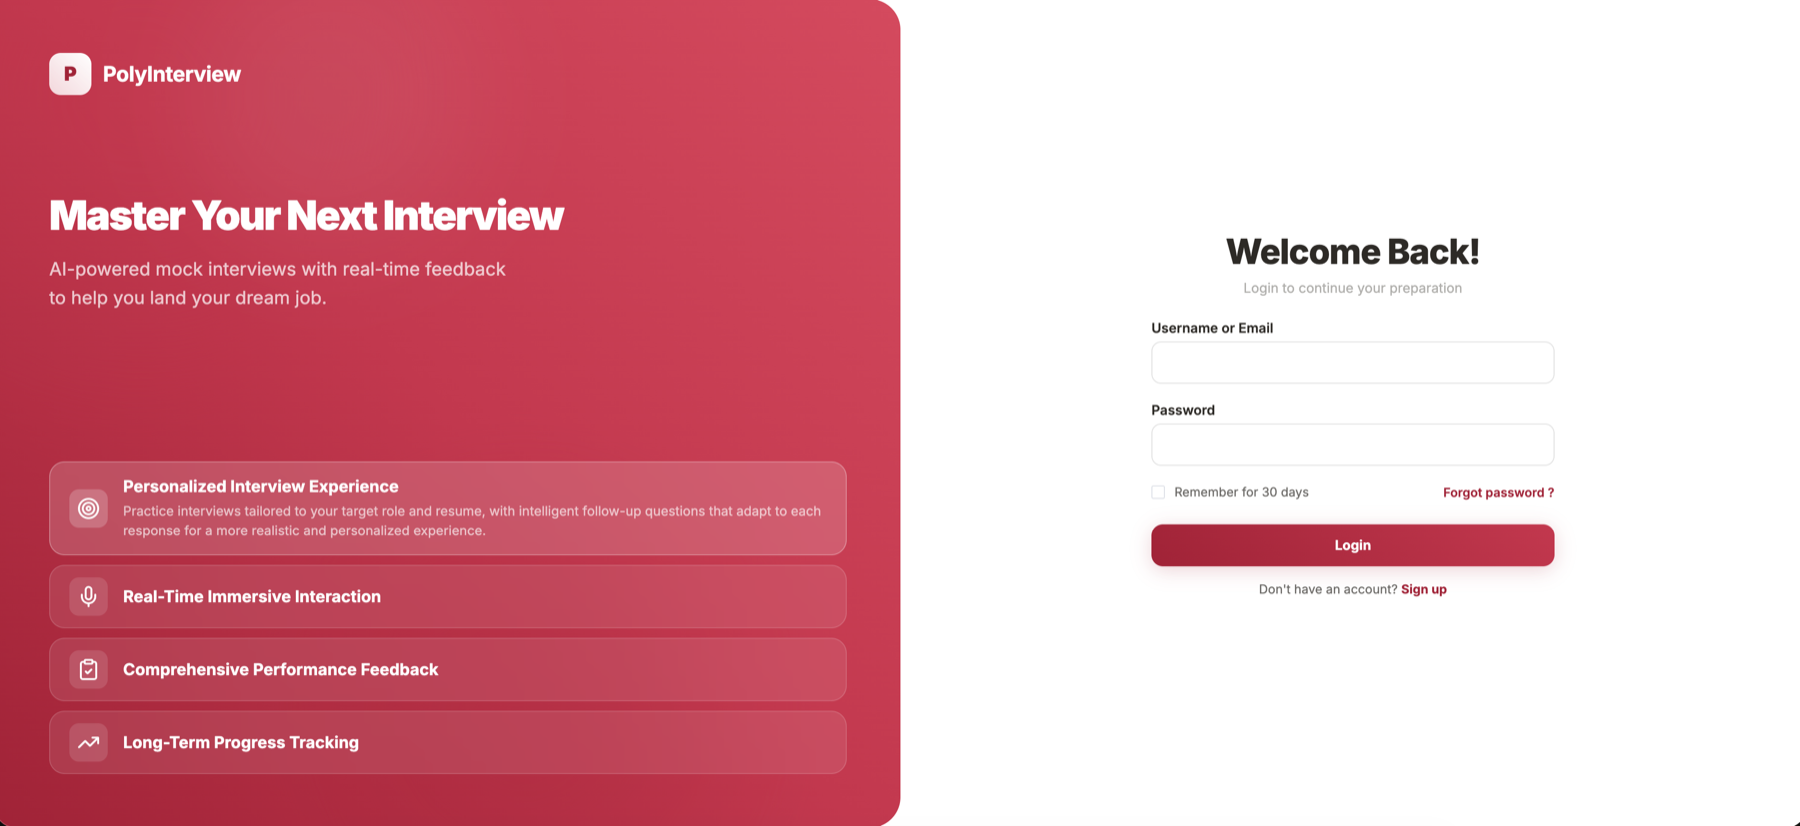
\includegraphics[width=\linewidth]{figures/ui/login.png}
    \caption{Landing / sign-in: the four pillars a student is promised.}
    \label{fig:ui-login}
  \end{subfigure}\hfill
  \begin{subfigure}[t]{0.485\textwidth}
    \centering
    
\includegraphics[width=\linewidth]{figures/ui/setup.png}
    \caption{Setup: interviewer persona, target role + JD, duration, and CV, all on one screen.}
    \label{fig:ui-setup}
  \end{subfigure}

  \vspace{5pt}
  \begin{subfigure}[t]{0.485\textwidth}
    \centering
    
\includegraphics[width=\linewidth]{figures/ui/live.png}
    \caption{Live interview: a lip-synced digital human (left) and the candidate's synchronized capture (right).}
    \label{fig:ui-live}
  \end{subfigure}\hfill
  \begin{subfigure}[t]{0.485\textwidth}
    \centering
    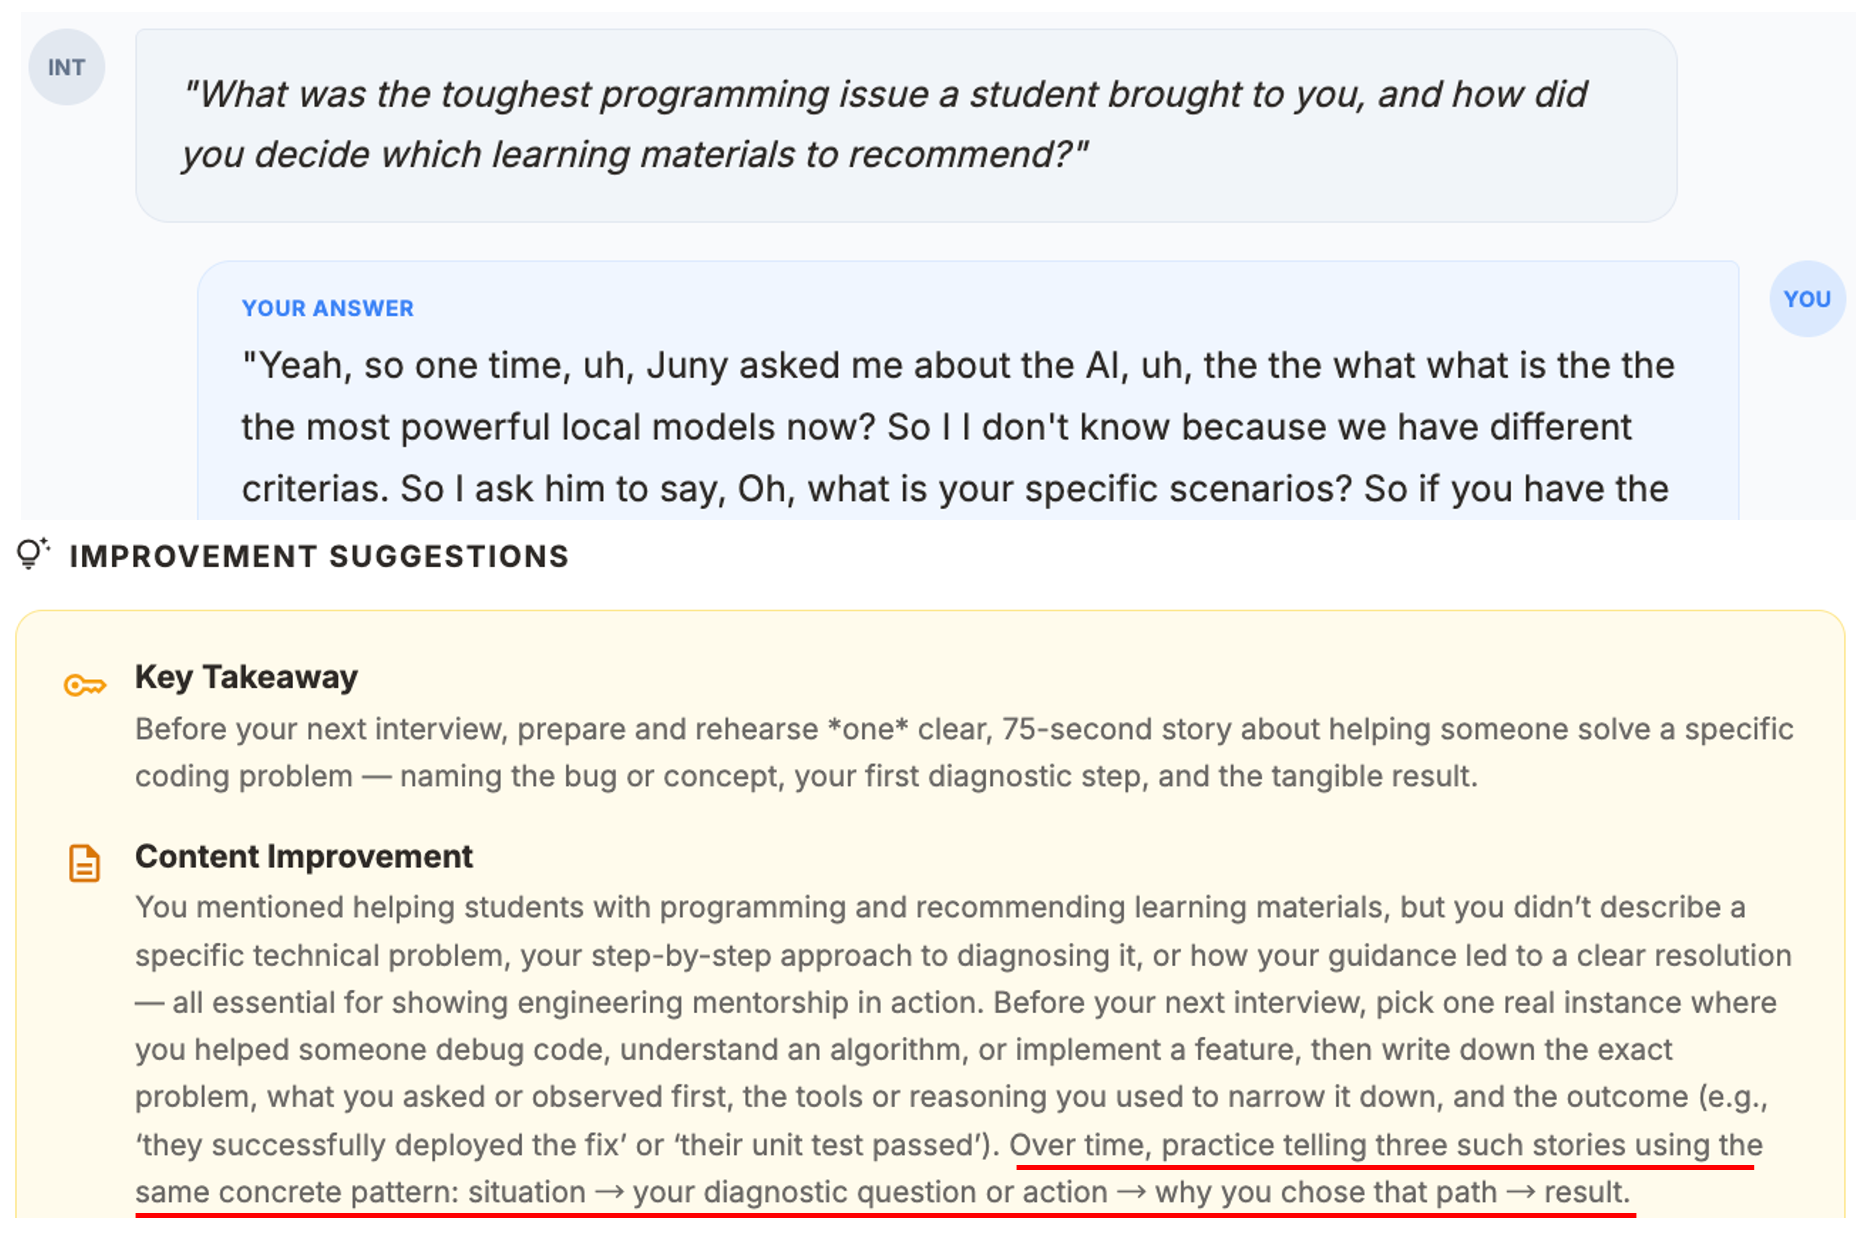
\includegraphics[width=\linewidth]{figures/ui/feedback_q.png}
    \caption{Per-question replay: score, transcript, and an AI-polished version of the student's \emph{own} answer.}
    \label{fig:ui-feedback}
  \end{subfigure}
  \caption{The end-to-end student experience, one screen per stage. A candidate signs in (\ref{fig:ui-login}), configures a session in a single form (\ref{fig:ui-setup}), talks to an embodied interviewer that also records voice, face, and posture (\ref{fig:ui-live}), and then replays each answer with a score and a rewritten model version (\ref{fig:ui-feedback}). The whole-interview report is shown separately in Figure~\ref{fig:report}.}
  \label{fig:journey}
\end{figure*}

\paragraph{Getting in and setting up.} The landing screen states the platform's four pillars: a personalized interview experience, real-time immersive interaction, comprehensive performance feedback, and long-term progress tracking (Figure~\ref{fig:ui-login}). Setup then fits an entire interview configuration onto one screen (Figure~\ref{fig:ui-setup}). The student picks one of three interviewer avatars, selects a target role from a set of company/position presets or types a custom one with its job description, uploads a CV (PDF or DOCX, parsed on the fly), and chooses an 8-, 15-, or 30-minute session, which the system maps to a proportionally larger question count. There is no prompt to write; the form \emph{is} the interface to a personalization pipeline.

\paragraph{Embodied live interview.} The interviewer is a lip-synced digital human (Wav2Lip; \citealp{prajwal2020wav2lip}) streamed to the browser over WebRTC, with speech synthesis and streaming recognition for a spoken exchange; avatars differ in face, voice, and tone. The live screen puts the avatar and the candidate side by side (Figure~\ref{fig:ui-live}), with a connection indicator, a per-session progress bar, and a single \textsc{Start Answering} control, so the interaction reads like a video call rather than a form. Talking to a face restores the social pressure that flat-text practice cannot. Voice, expression, and posture stream in together and are recorded per question, so the system can later judge not just \emph{what} a candidate says but \emph{how}.

\paragraph{Two-tier feedback.} Feedback is delivered at two granularities. After each answer, a per-question replay (Figure~\ref{fig:ui-feedback}) shows a 0--10 score, the full conversation flow, and, next to the student's raw transcript, an \emph{AI-suggested answer} that rewrites their own words into a higher-scoring version with the same content. In one recorded self-introduction, a hesitant ``\emph{Um. Okay. So um. My name is Zhiyuan\ldots and a I in the.}'' is rewritten into a fluent, structured paragraph that keeps every fact the student supplied, so the lesson is phrasing rather than new material. When the session ends, a whole-interview report (\S\ref{sec:scoring}, Figure~\ref{fig:report}) integrates an overall verdict, the two competency scores, a radar over ten aspects, and a panel of thirteen multimodal features, and exports to PDF. The loop is deliberately pedagogical: each answer becomes the material for the next, better one.

\paragraph{At the demo.} A booth visit runs the same loop in a few minutes. A visitor picks an interviewer persona and either uploads a CV or uses a bundled sample CV and job description, holds a short spoken exchange of three or four questions with the digital human, and then we open their report and follow one score from the overall verdict to the ten-aspect radar down to a single feature and its practice tip, which is the traceability we most want people to feel. The live avatar runs on our own machine through the session pool (five concurrent sessions, queued when full); because a booth network is unreliable and the system itself fails on some webcam captures, we also carry a pre-recorded end-to-end session and an exported PDF report as an offline fallback.

\section{Adaptive Multi-Agent Questioning}
\label{sec:match}

The \textsc{Match} side asks whether the candidate's ability fits the role, and it is driven by two cooperating agents whose behavior is visible in the setup and live screens above.

\begin{figure}[t]
  \centering
  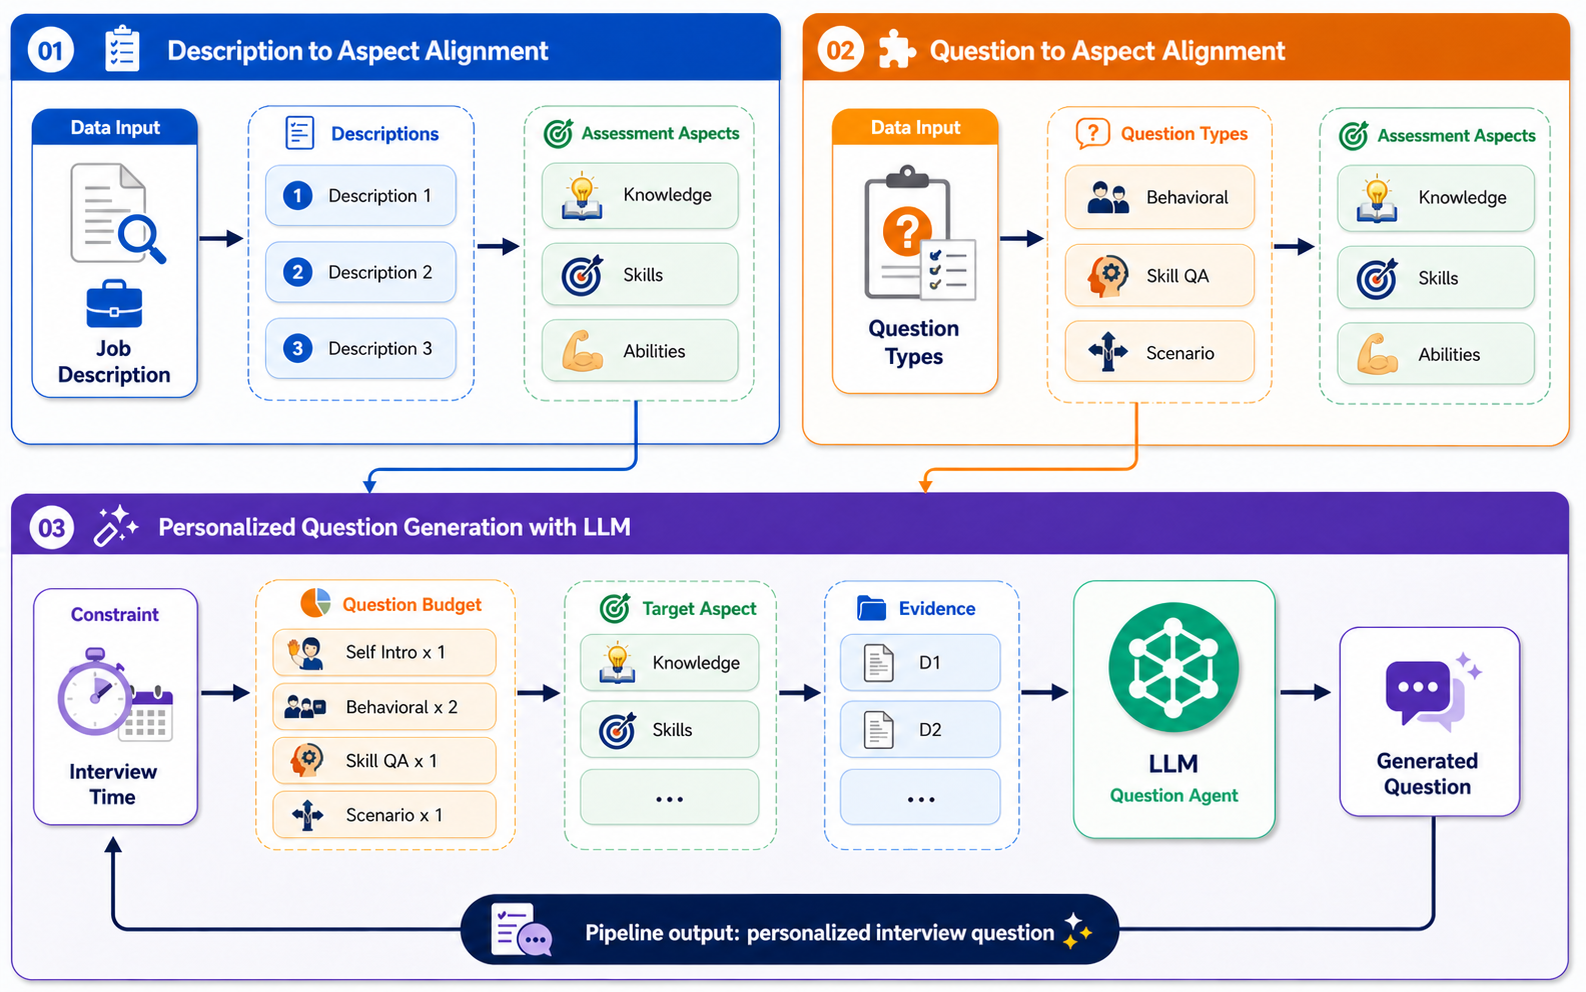
\includegraphics[width=\linewidth]{figures/flow/question_generation.png}
  \caption{Personalized question generation. Two alignment stages map the job description and the question type to KSA-scored assessment aspects; a question-budget derived from the chosen duration then drives an LLM agent that generates each item from the aligned aspects and CV evidence.}
  \label{fig:qgen}
\end{figure}

\paragraph{Planning the interview.} An \emph{Interview Planner Agent} reads the job description, interviewer profile, duration, and CV, and produces a structured question list spanning self-introduction, behavioral, skill-QA, and scenario stages (Figure~\ref{fig:qgen}). Two alignment stages map first the job description and then each question type onto the KSA-aligned assessment aspects (\S\ref{sec:scoring}); a question budget derived from the session length allocates how many items each stage gets, and an LLM question agent writes each item from the aligned aspects and concrete CV evidence. The result is a session that is personalized before the first word is spoken, and personalized \emph{to the rubric it will later be scored against}.

\begin{figure}[t]
  \centering
  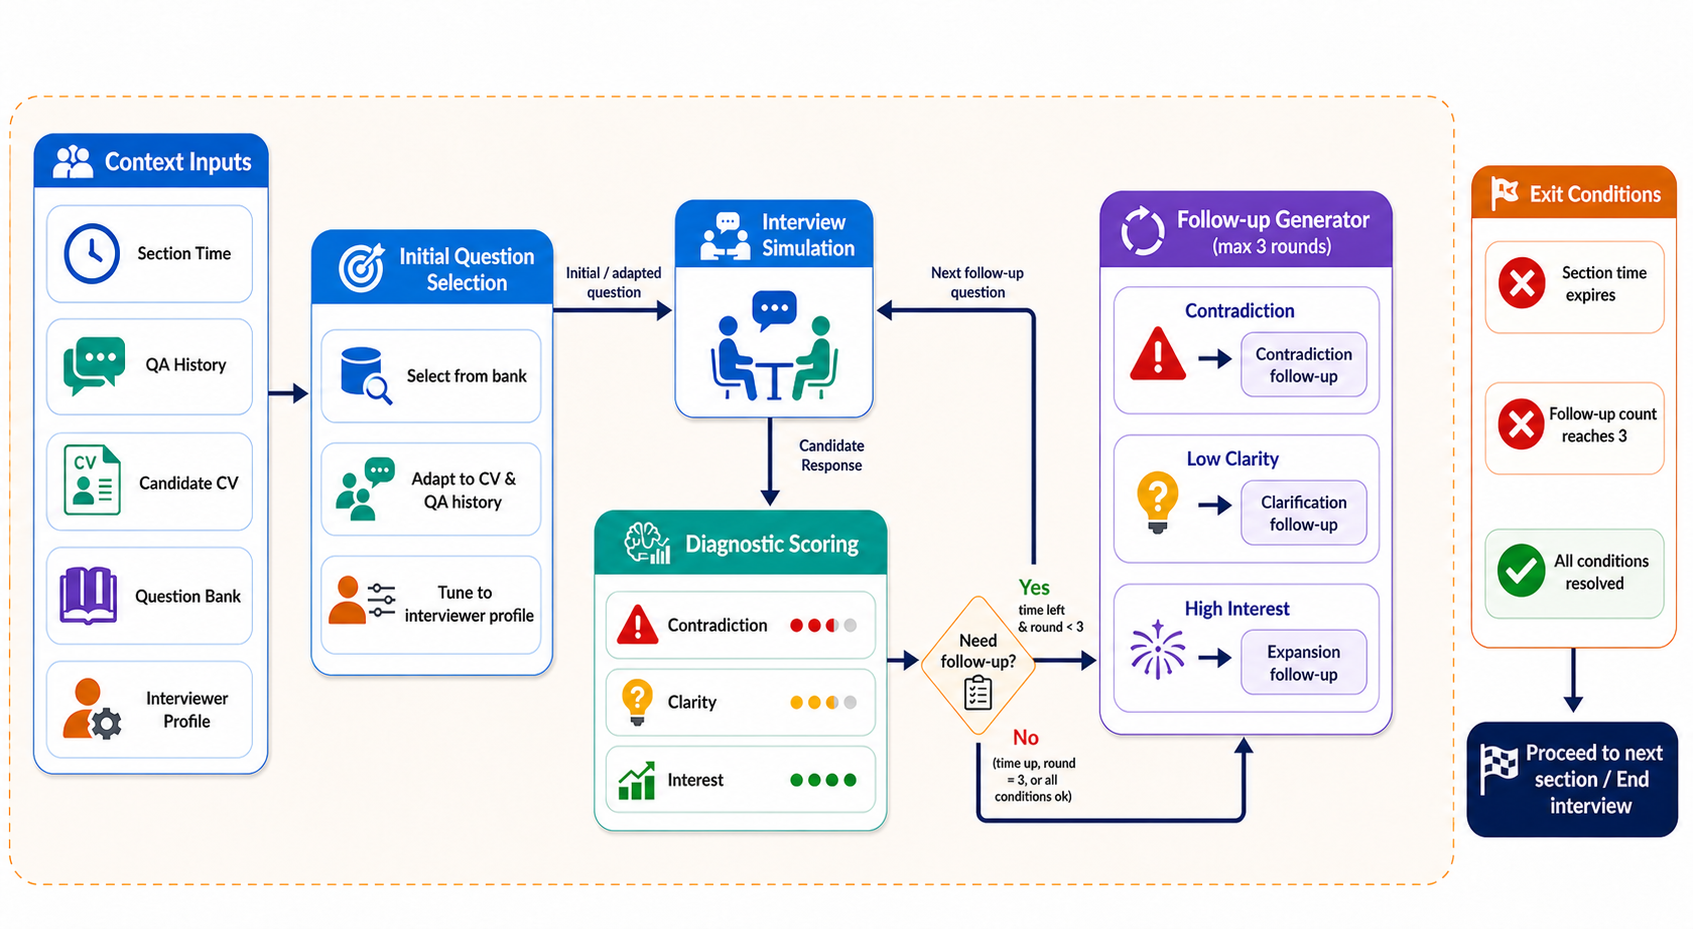
\includegraphics[width=\linewidth]{figures/flow/adaptive_followup.png}
  \caption{Real-time adaptive follow-ups. After each answer a diagnostic agent scores contradiction, clarity, and interest; a controller either issues a targeted follow-up (contradiction, clarification, or expansion) or moves on. Probing is bounded by section time and a per-question follow-up cap.}
  \label{fig:followup}
\end{figure}

\paragraph{Following up in real time.} An \emph{Interviewer Agent} asks each question in the chosen style and, after every answer, runs a Response-Check that rates the answer for consistency, clarity, and relevance (operationalized in Figure~\ref{fig:followup} as contradiction, clarity, and interest) and emits a follow-up signal: probe again, or move on. A contradiction triggers a contradiction follow-up, a vague answer a clarification follow-up, and a strong answer an expansion that pushes toward trade-offs; the loop exits when section time runs out, the follow-up cap is reached, or the answer resolves. The three interviewer personas bind style to depth: Amy (Basic) asks at most one follow-up, David (Intermediate) two, and James (Advanced) three, so the challenge scales with the candidate and personalization continues past the opening question. Ask a database candidate ``how would you keep a checkout fast under load,'' and a vague answer draws a follow-up on indexing while a crisp one is pushed toward consistency trade-offs.

\section{Explainable Multimodal Scoring}
\label{sec:scoring}

\begin{figure}[t]
  \centering
  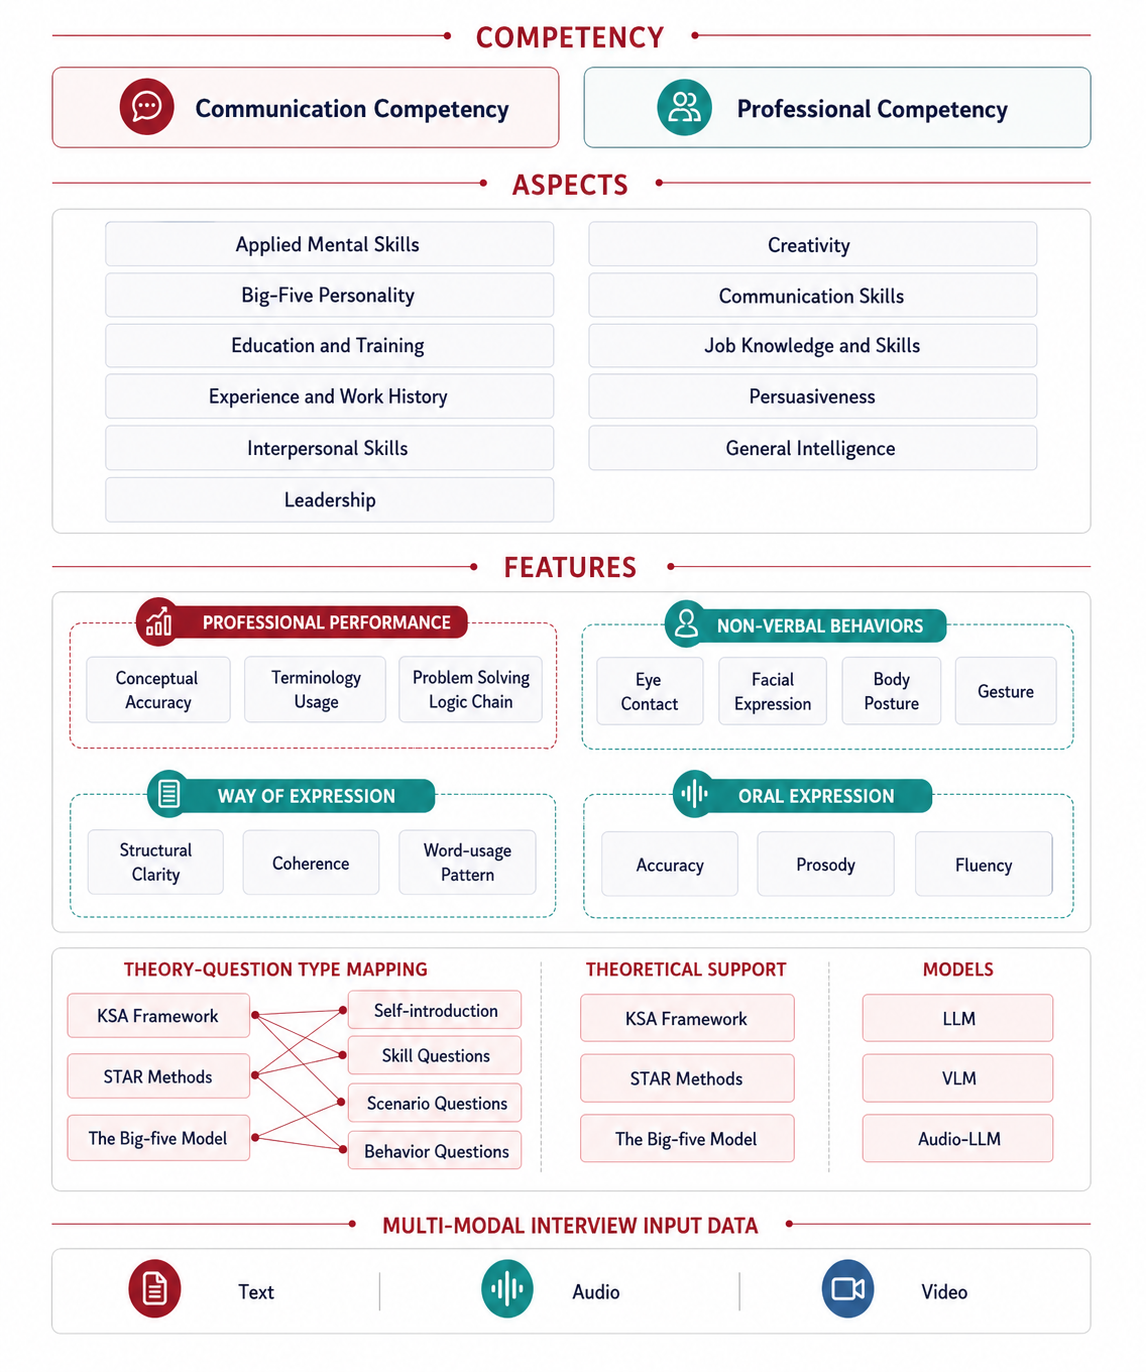
\includegraphics[width=\linewidth]{figures/flow/assessment_framework.png}
  \caption{The three-layer evaluation framework, bottom to top. Multimodal input (text, audio, video) feeds four feature agents that produce thirteen features; an aggregation step maps them to the ten KSA-aligned aspects under question-type gating (the Big-Five model grounds the social family), and aspects roll up into two competency tracks. KSA, STAR, and Big-Five provide the theoretical grounding; each layer is scored by an LLM, VLM, or audio model. Every score traces back across the layers to the behavioral signal that produced it.}
  \label{fig:arch}
\end{figure}

PolyInterview scores the \textsc{Convince} side with the three-layer architecture in Figure~\ref{fig:arch}. The four feature agents run concurrently (through a thread pool) on each answer, so a full interview is scored in roughly the compute of a single answer rather than as a separate batch pass.

\paragraph{Layer 1: Features.} Thirteen 0--10 signals come from four agents that run together on each answer. A \emph{Professional-Performance} agent (LLM, text) rates conceptual accuracy, terminology use, and the problem-solving logic chain. A \emph{Way-of-Expression} agent (LLM, text) rates structural clarity, coherence, and word-usage pattern. A \emph{Non-verbal-Behavior} agent (a Qwen-VL-family vision-language model; \citealp{bai2023qwenvl}) rates eye contact, facial expression, body posture, and gesture from the recorded video. An \emph{Oral-Expression} agent (speech) rates pronunciation accuracy, prosody, and fluency from the audio.

\paragraph{Layer 2: Aspects.} An aggregation agent maps the features onto ten KSA-aligned aspects in three families: \emph{cognitive} (general intelligence, applied mental skills, creativity), \emph{background} (job knowledge and skills, education and training, experience and work history), and \emph{social} (communication, interpersonal skills, leadership, persuasiveness), the last aligned with the Big-Five factors \citep{mccrae1987validation}. Each aspect is a 70/30 weighting of primary and secondary features. Only the aspects \emph{relevant} to a question type are scored: a behavioral question activates interpersonal skills, applied mental skills, and leadership, while a skill-QA question activates job knowledge, general intelligence, and education. Teamwork is never scored on a question that cannot elicit it; the complete aspect--feature mapping and per-type gating are in Appendix~\ref{app:mapping}.

\paragraph{Layer 3: Proficiency.} Aspects roll up into Professional Competency (cognitive plus background) and Communication Competency (social), and the overall score is their mean; a CV-informed step tailors the improvement suggestions to the candidate's background.

\paragraph{Theory grounding.} Two established hiring frameworks keep the scores interpretable. KSA names \emph{what} we assess and drives the professional track; each K/S/A binds to a feature a language, vision, or speech agent can detect. STAR (Situation, Task, Action, Result) names \emph{how} a candidate should answer and drives the communication track, a structure with roots in behavior-description interviewing \citep{janz1982behavior}; a missing Result yields a concrete prompt to add one, and because students are scored against the structure they are taught, the feedback is directly usable. No score is a dead end: it traces from proficiency through aspect to the feature and modality that moved it.

\begin{figure*}[t]
  \centering
  \begin{subfigure}[t]{0.49\textwidth}
    \centering
    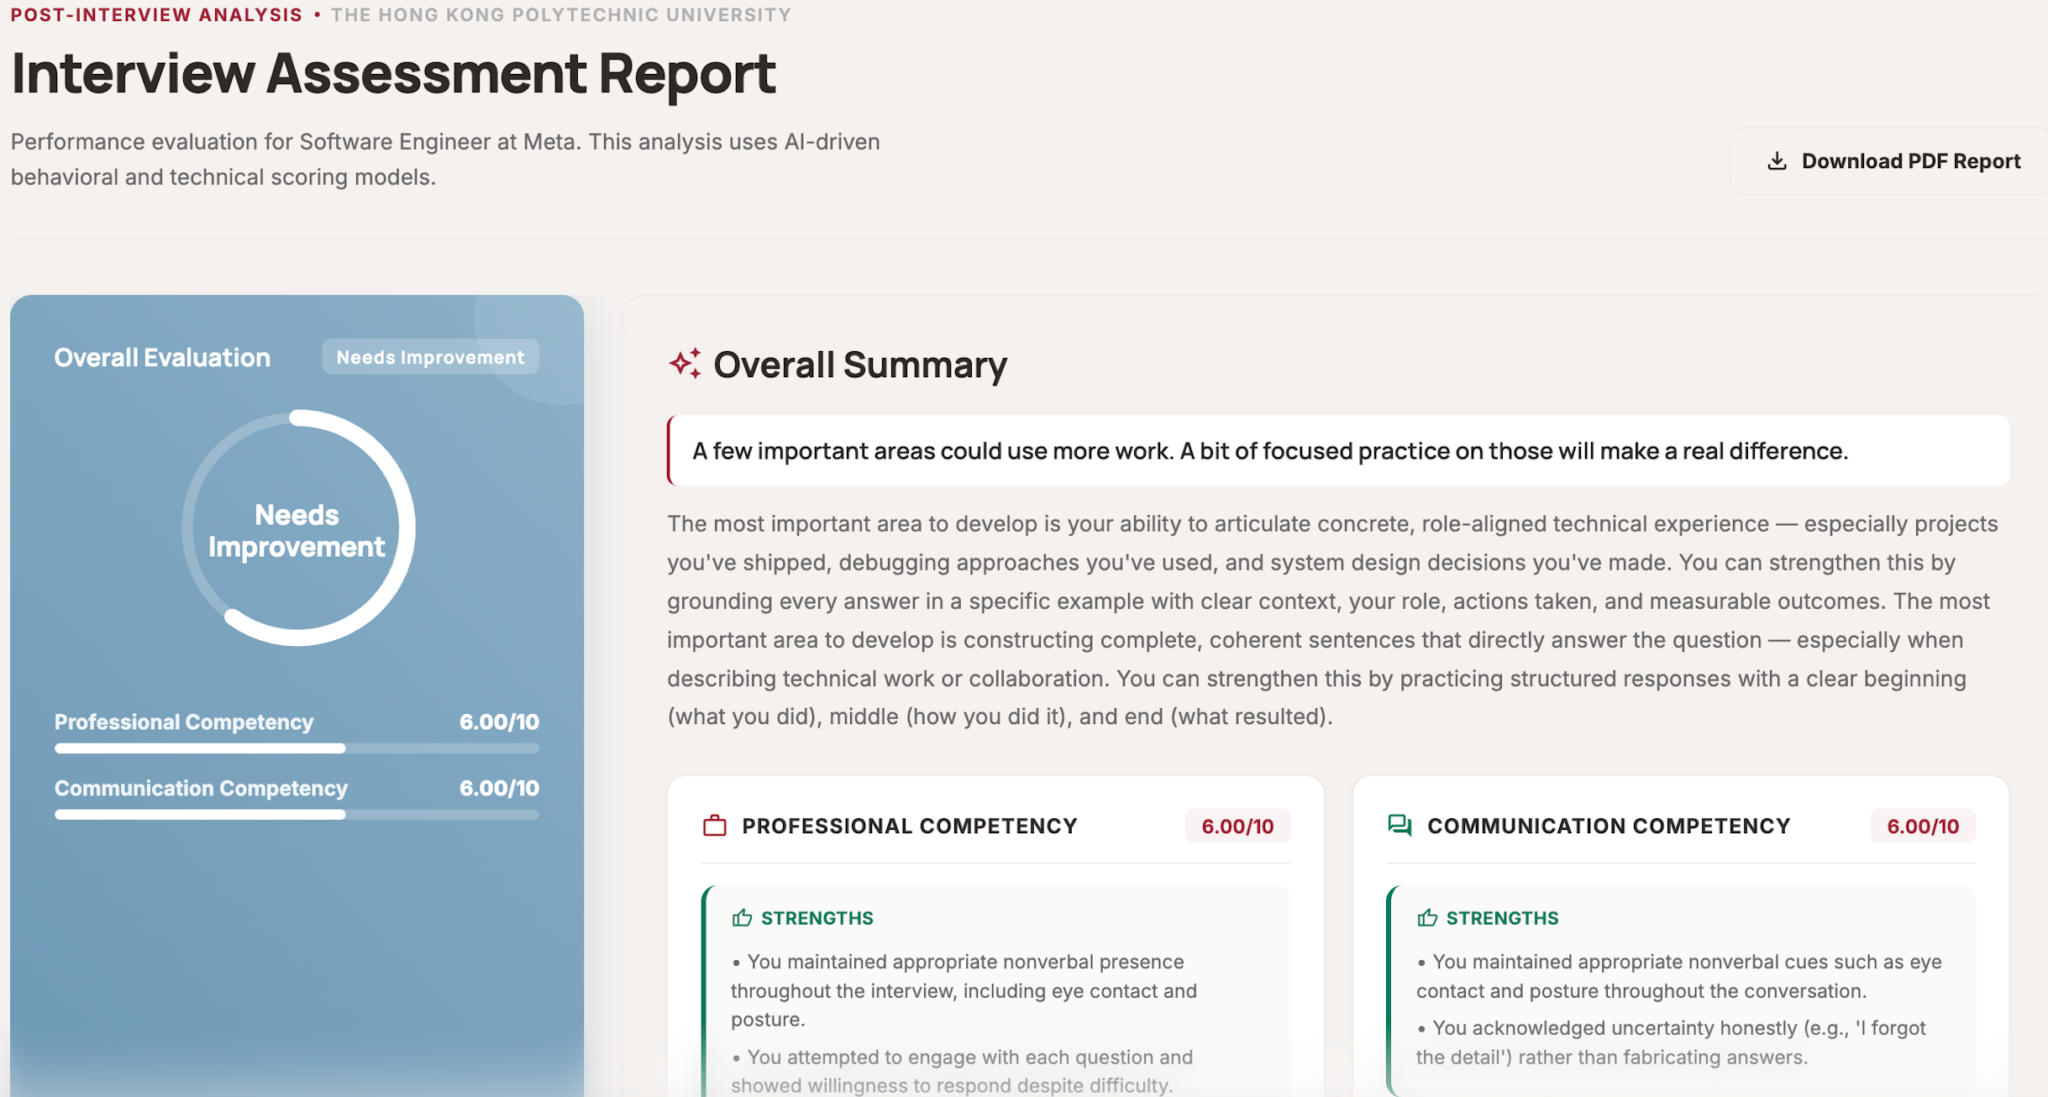
\includegraphics[width=\linewidth]{figures/ui/report_overall.png}
    \caption{Overall report: a verdict, the two competency scores, and a written summary, exportable to PDF.}
    \label{fig:report-overall}
  \end{subfigure}\hfill
  \begin{subfigure}[t]{0.49\textwidth}
    \centering
    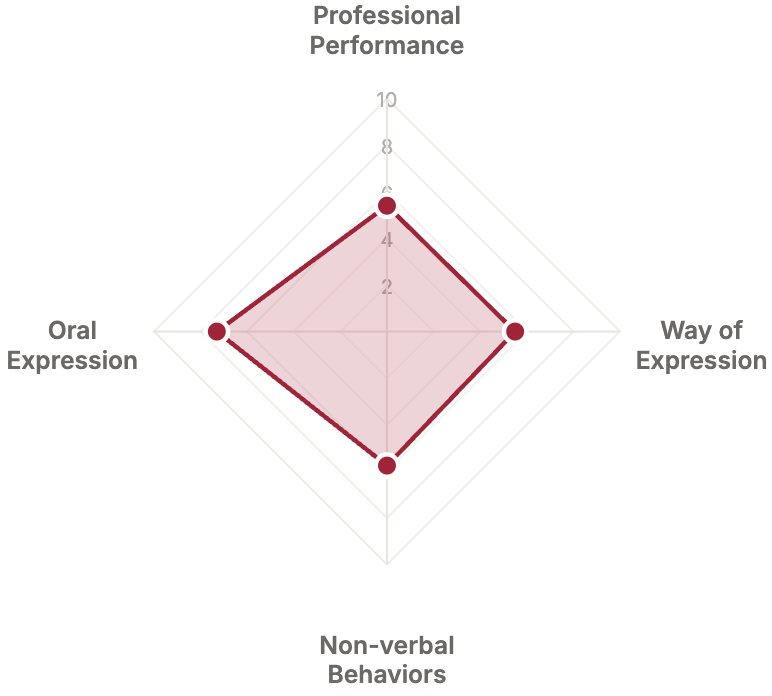
\includegraphics[width=\linewidth]{figures/ui/skills.png}
    \caption{Skills \& behaviors breakdown: each feature expands into a score, a diagnosis, and a concrete practice tip.}
    \label{fig:report-skills}
  \end{subfigure}

  \vspace{5pt}
  \begin{subfigure}[t]{0.92\textwidth}
    \centering
    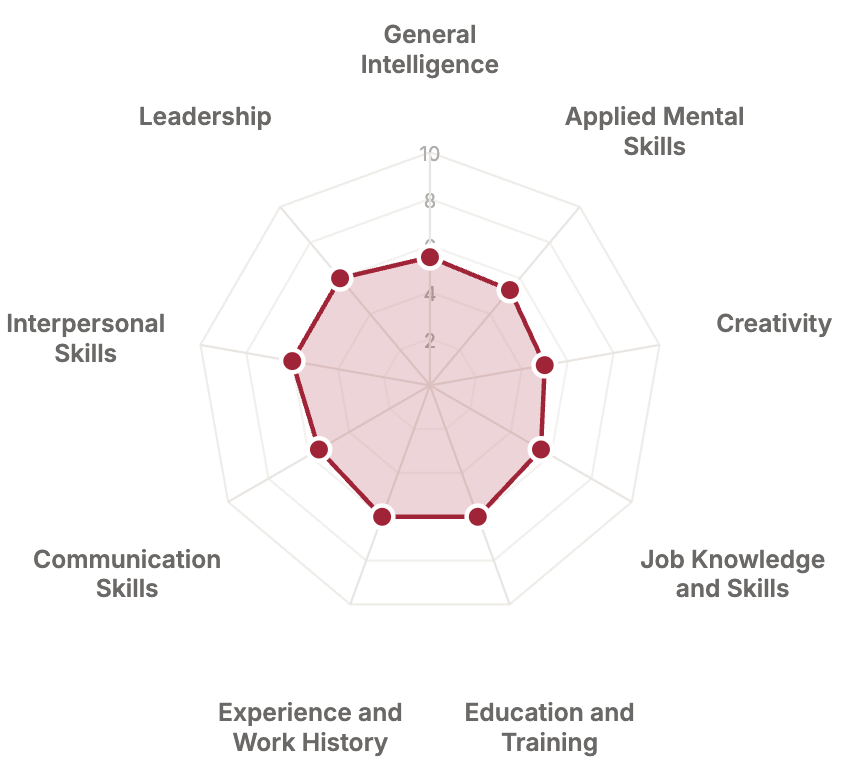
\includegraphics[width=\linewidth]{figures/ui/competency.png}
    \caption{Competency overview: a radar over the KSA-aligned aspects activated for this session (question-type gating means not all ten appear every time), each with a diagnosis and an actionable tip.}
    \label{fig:report-radar}
  \end{subfigure}
  \caption{The explainable report makes traceability tangible. The overall verdict (\ref{fig:report-overall}) drills down into the aspect radar (\ref{fig:report-radar}) and further into the thirteen features (\ref{fig:report-skills}). The three panels are illustrative report screens from different demo sessions, shown to convey the interface rather than any single result, and are separate from the deployment corpus of \S\ref{sec:deploy}. Every number on screen is expandable to the behavioral signal beneath it and paired with a suggestion the student can act on.}
  \label{fig:report}
\end{figure*}

\paragraph{The report makes traceability tangible.} The whole-interview report is where the layered design pays off for the user (Figure~\ref{fig:report}). The top level is a single verdict and the two competency scores (Figure~\ref{fig:report-overall}); one level down, a radar plots the activated aspects, each with a short diagnosis and a concrete tip (Figure~\ref{fig:report-radar}); one level further, the thirteen features expand individually, so a low \emph{Eye Contact} is not just a number but a sentence explaining it and a specific practice drill (Figure~\ref{fig:drilldown}). Because visual scoring stays advisory and always shows its evidence, the interface embodies the responsible-use stance we argue for in \S\ref{sec:related} and the Ethics Statement.

\begin{figure}[t]
  \centering
  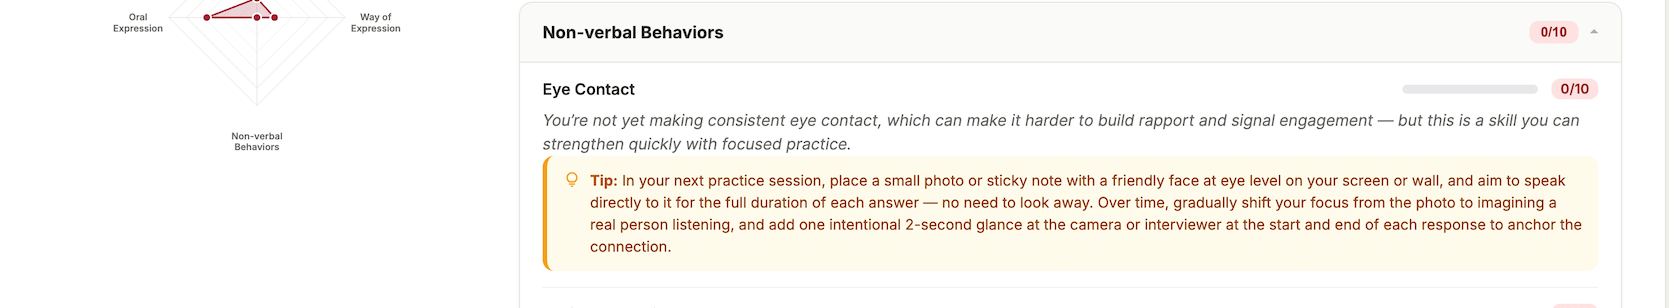
\includegraphics[width=\linewidth]{figures/ui/drilldown.png}
  \caption{One feature, read end to end. The report expands \emph{Eye Contact} into a 0/10 score, a plain-language diagnosis, and a specific practice drill; the left radar keeps it in context. This drill-down is what ``traceable'' means at the interface, and it is what a visitor sees for their own answer at the demo.}
  \label{fig:drilldown}
\end{figure}

\paragraph{Implementation.} The frontend is a Vue.js single-page app (Vue 2.6 + Element UI); a Flask API orchestrates interview flow and evaluation, and a separate Node/Express service handles authentication (Prisma + SQLite, bcrypt, 7-day JWT). Text scoring uses Qwen-Plus/Qwen-Flash via DashScope (switchable to GPT-4o through the OpenAI SDK); non-verbal analysis uses Qwen3-VL-Plus (in the Qwen-VL family; \citealp{bai2023qwenvl}), streaming recognition uses a real-time Qwen3-ASR model, speech synthesis uses Edge-TTS (Azure backup), and pronunciation scoring uses the Azure Speech SDK. The digital human (LiveTalking + Wav2Lip) streams over WebRTC via aiortc, and the platform runs as four cooperating services (frontend, API, auth, digital-human) behind HTTPS with a session pool that caps concurrency at five and queues when full.

\section{Deployment and What It Reveals}
\label{sec:deploy}

\begin{table}[t]\centering\small
\begin{tabular}{@{}p{0.67\linewidth}r@{}}
\toprule
\textbf{Statistic} & \textbf{Snapshot} \\
\midrule
Accounts & 101 \\
Returning accounts & 62 \\
Sessions & 1{,}564 \\
Generated questions & 7{,}665 \\
Completed sessions & 217 \\
Five-stage question sets & 1{,}422 \\
Distinct position titles & 83 \\
Answered question records & 1{,}274 \\
Recorded follow-up turns & 342 \\
Pooled scored answers & 1{,}425 \\
Audio/video files (wav/webm) & 1{,}744 / 1{,}754 \\
\bottomrule
\end{tabular}
\caption{All-account usage snapshot, including internal and test activity.}
\label{tab:deploy}
\end{table}


\paragraph{Deployment and corpus.} PolyInterview runs on the university network. The raw logs span 85 accounts and 1{,}535 sessions (14\,GB of text, audio, video, and CVs), but most of that volume is testing: a single \texttt{Test User} account holds 369 sessions, and integer-seed and junk accounts hold hundreds more. Four explicit rules (explicit ``test'' naming, internal integer-seed IDs, junk or placeholder names, and research-team self-tests) remove 39 accounts and leave \textbf{46 genuine users, 120 sessions, and 475 recordings} (Table~\ref{tab:deploy}); each answer is captured as WebM with an extracted WAV track of identical duration and is transcoded to MP4. We use this cleaned set as our analysis corpus and do not report the contaminated numbers, which tell a different and more flattering story. The 46 genuine users here are the campus deployment's logged users; the two-round pilot in \S\ref{sec:eval} draws on a separate, broader pool of 129 participants across six institutions that overlaps them only in part.

\begin{figure}[t]
  \centering
  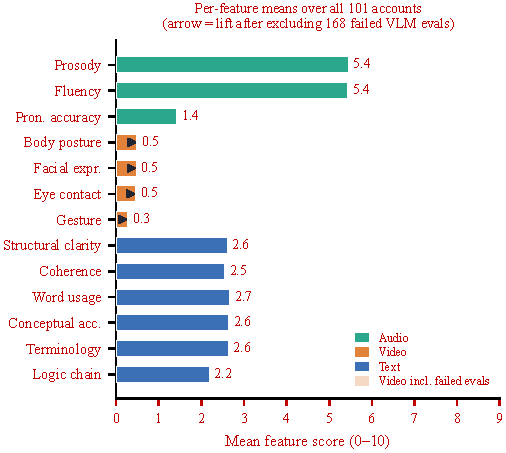
\includegraphics[width=\linewidth]{figures/fig_modality.pdf}
  \caption{Mean of each feature over the cleaned corpus, by modality. Audio (prosody, fluency) scores leniently high; text content sits near the floor on mostly short answers. For the four video features, the arrow marks the lift once the 74 silent zero-returns are excluded; the 106 no-video answers are still counted, so this is a failure-only, conservative correction.}
  \label{fig:modality}
\end{figure}

\begin{figure}[t]
  \centering
  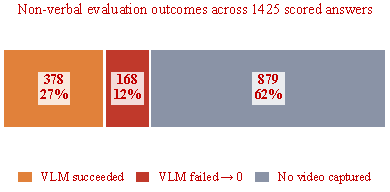
\includegraphics[width=\linewidth]{figures/fig_reliability.pdf}
  \caption{Outcomes of the non-verbal (video) evaluator across the 233 answers where a video score was expected. Only 22.7\% (53) yield a genuine score; on 31.8\% (74) there was video but the evaluator silently returned a zero, and 45.5\% (106) had no capturable video. Among just the 127 answers with captured video, the evaluator silently failed on 58\%. The per-feature architecture is what makes this visible.}
  \label{fig:reliability}
\end{figure}

\paragraph{The architecture surfaces its own failure mode.} Because every score is traceable to a feature and modality, aggregating over the cleaned corpus does more than rank features; it audits the evaluator. Two things stand out (Figure~\ref{fig:modality}). First, audio features score leniently high (prosody and fluency near $6.6/10$) while text-content features sit near the floor, consistent with a corpus of mostly short, partly abandoned walk-up sessions (text content spans $0.76$--$1.12$; overall scores are zero-inflated, and among non-zero sessions the mean is only $1.76$ and the maximum $4.80$). Second, and more useful, the video features look low for a reason the architecture exposes: the non-verbal evaluator \emph{silently fails}, recording a zero, on $31.8\%$ of the $233$ answers where a video score was expected (and on $58\%$ of the $127$ that actually had captured video), with another $45.5\%$ having no capturable video and only $22.7\%$ producing a genuine score (Figure~\ref{fig:reliability}). Excluding the failures lifts the video means by roughly $44\%$ (eye contact $1.11\!\rightarrow\!1.60$, posture $1.15\!\rightarrow\!1.66$). The headline ``vision scores lowest'' is therefore partly an artifact of unreliable inference on real, noisy webcam video, a diagnosis we could make only because each feature is reported separately rather than folded into one number.

\paragraph{Modalities carry non-redundant signal.} Across sessions, the modality scores are weakly related (text--audio $r{=}0.40$, text--video $r{=}-0.14$, audio--video $r{=}-0.10$), so the channels carry largely non-redundant signal, which supports keeping the modalities separate in analysis rather than collapsing them into one number; it does not by itself validate the scores. The $31.8\%$ silent-failure rate is a separate matter: an engineering defect to fix at the source (retries, a fallback model, capture-quality checks), not something the other channels can paper over.

\begin{figure}[t]
  \centering
  \begin{subfigure}[t]{0.5\linewidth}
    \centering
    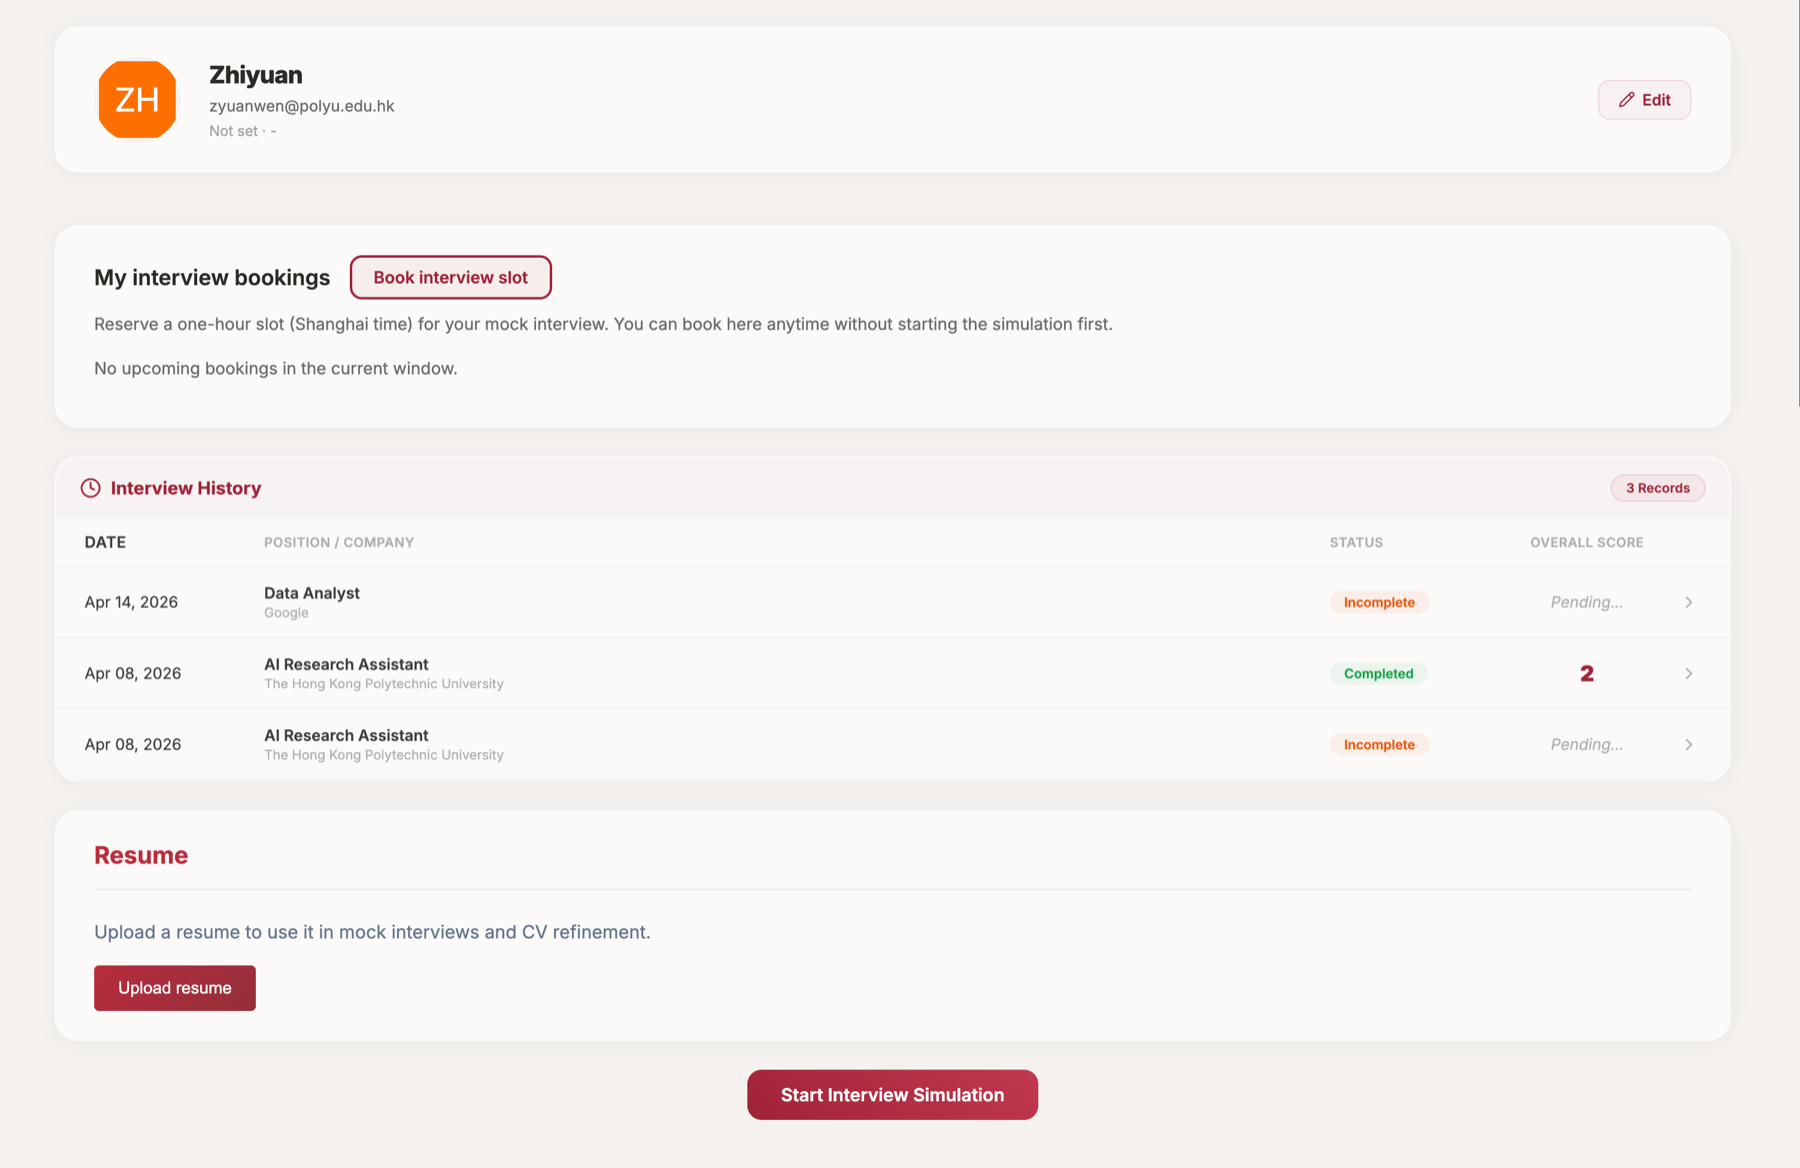
\includegraphics[width=\linewidth]{figures/ui/dashboard.png}
    \caption{Account dashboard: history, scores, bookings, CV.}
    \label{fig:ui-dashboard}
  \end{subfigure}\hfill
  \begin{subfigure}[t]{0.46\linewidth}
    \centering
    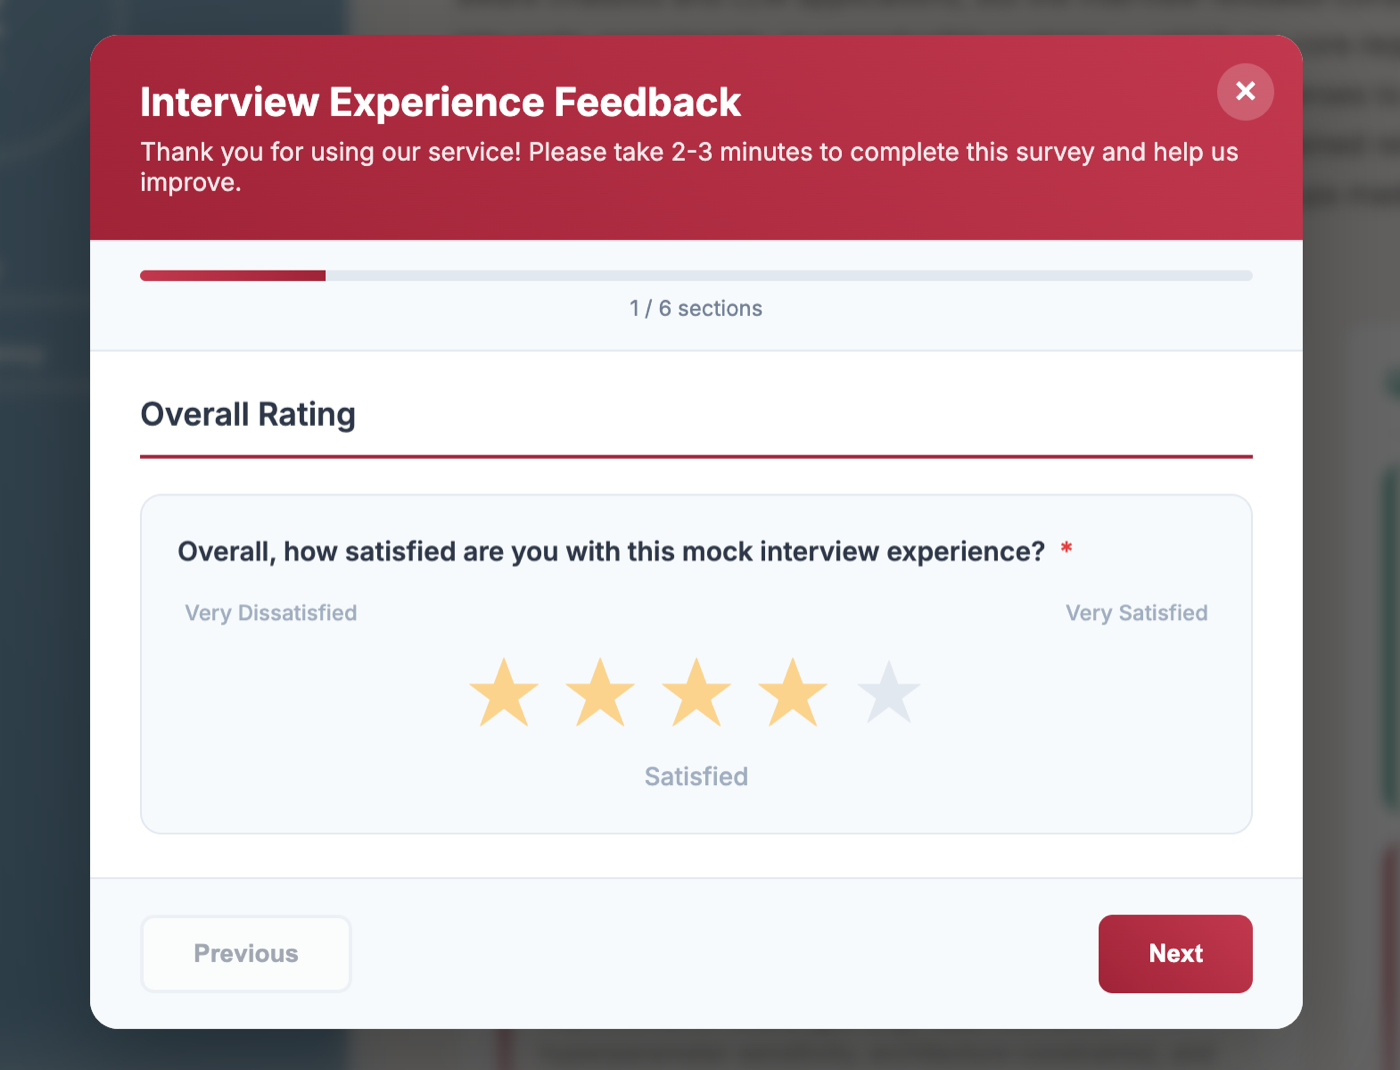
\includegraphics[width=\linewidth]{figures/ui/survey.png}
    \caption{In-app experience survey.}
    \label{fig:ui-survey}
  \end{subfigure}
  \caption{Deployment support. A per-user dashboard tracks interview history, scores, one-hour booking slots, and the stored CV (\ref{fig:ui-dashboard}); an optional in-app survey collects the self-report feedback summarized in \S\ref{sec:eval} (\ref{fig:ui-survey}).}
  \label{fig:deploy-ui}
\end{figure}

\paragraph{Progress tracking and booking.} Each account has a dashboard (Figure~\ref{fig:deploy-ui}) that lists past sessions with their status and overall score, exposes the built-in one-hour booking function, and stores a reusable CV (Figure~\ref{fig:ui-dashboard}), which is what turns a one-off practice run into the ``long-term progress tracking'' promised on the landing screen. An optional in-app survey (Figure~\ref{fig:ui-survey}) is how we collected the self-report feedback below.

\section{Evaluation}
\label{sec:eval}
\paragraph{Pilot user study.} Across two rounds we gathered feedback from 129 participants spanning six institutions and eight-plus disciplines, including nine faculty reviewers from English-language teaching units. A broad first round endorsed the core experience (UI clarity 67\%, immersive digital interviewer 58\%, report depth 50\%, personalized questions 42\%), and deeper second-round interviews with senior students preparing technical interviews consistently reported that the flow was smooth enough for real practice, the questions felt professional and on-topic, and the digital interviewer felt close to a real session. These are self-reports, and we treat them as such.

\paragraph{Planned validation.} The deployment analysis points to what to measure next, and the explainable design makes each measurable. \emph{(i) Reliability.} We will report the non-verbal evaluator's failure rate as a first-class metric and drive it down with retries, a fallback model, and capture-quality checks; Figure~\ref{fig:reliability} is the baseline. \emph{(ii) Criterion validity.} We will collect blinded ratings from career-service experts on a stratified sample of recorded answers and measure agreement with the system per aspect (intraclass correlation and Krippendorff's $\alpha$), which the current self-report evidence cannot establish. \emph{(iii) Learning gain.} A pre/post design (a baseline mock interview, a block of PolyInterview practice, then a fresh interview scored by blinded experts) will test whether practice transfers, with an arm that toggles adaptive follow-ups to isolate their effect. These run in stages (reliability now, criterion validity next term, the learning-gain study after), alongside standardized usability and workload instruments (the System Usability Scale and Raw NASA-TLX) for active users, moving the system from ``well received'' toward ``measured.''

\section{Conclusion}
PolyInterview is a deployed, multi-agent mock-interview system that pairs adaptive, personalized questioning with multimodal, theory-grounded, and traceable feedback, delivered through an interface a student can walk through end to end at the demo. It is live, has reached students across six institutions through a two-round pilot, and because every score points back to a behavioral signal, its own deployment data exposes where the evaluation is weak, starting with a non-verbal evaluator that fails silently on a third of answers. That traceability is the contribution we would most like reviewers and users to experience at the live demo: a score you can follow back to the moment that produced it.

\section*{Limitations}
The deployment evaluation is observational and self-reported; we do not yet report agreement between system scores and blinded expert ratings, which \S\ref{sec:eval} is designed to fix. The cleaned deployment corpus analyzed here is modest (120 sessions, with a smaller effective sample once zero-score abandoned sessions are set aside), English-centric, and drawn from a single institution's network, even though the pilot study and broader user base span six institutions; the descriptive numbers should not be read as population estimates. The report screens in Figure~\ref{fig:report} are illustrative interface walkthroughs from different demo sessions, not evidence of typical performance. The non-verbal failure rate we report is itself a moving target that depends on webcam quality and model availability. Finally, parts of the pipeline call external model providers under no-training terms; full on-campus inference is in progress.

\section*{Ethics Statement}
PolyInterview is an advisory practice tool for students, explicitly not a hiring or gatekeeping system, and its scores are explainable and contestable. Automated assessment of non-verbal behavior has a documented history of fairness concerns; we therefore keep visual scoring advisory, expose the evidence behind every score (Figure~\ref{fig:report-skills}), avoid any pass/fail decision, and, as \S\ref{sec:deploy} shows, report rather than hide where that scoring is unreliable. Data is stored on the campus network with per-user isolation and bcrypt-hashed credentials and is deletable on demand; encryption at rest is on the deployment roadmap and not yet in place, which we state plainly. Any research use is de-identified and IRB-approved, consistent with GDPR and Hong Kong's PDPO; the analysis in this paper uses de-identified session metadata only.

\bibliography{references}

\appendix
\section{Aspect--Feature Mapping and Question Gating}
\label{app:mapping}
Every aspect score is a $70/30$ blend of primary and secondary features, so any score is reconstructable from the signals beneath it (Table~\ref{tab:mapping}). Only the aspects a question type can elicit are scored: \textbf{Self-Introduction} activates Communication Skills, Education \& Training, and Experience; \textbf{Behavioral} activates Interpersonal Skills, Applied Mental Skills, and Leadership; \textbf{Skill-QA} activates Job Knowledge, General Intelligence, and Education \& Training; \textbf{Scenario} activates Applied Mental Skills, Creativity, and Persuasiveness; \textbf{Candidate Questions} are not scored. As a worked example of traceability: when Professional Competency reads low, the report points to the feature that pulled it down (a Problem-Solving Logic Chain of $0.76$, say) while flagging a strong Prosody ($6.6$) as delivery that already works, so the student fixes answer structure rather than voice.

\begin{table}[h]
\centering\footnotesize
\setlength{\tabcolsep}{3pt}
\begin{tabular}{@{}p{1.55cm}p{2.65cm}p{2.6cm}@{}}
\toprule
\textbf{Aspect} & \textbf{Primary (70\%)} & \textbf{Secondary (30\%)} \\
\midrule
\multicolumn{3}{@{}l}{\emph{Cognitive}} \\
Gen.\ Intelligence & ConcAcc, Logic & Coher, Clarity \\
Applied Mental & Logic, ConcAcc & Clarity, Coher \\
Creativity & Logic, Word & ConcAcc, Coher \\
\midrule
\multicolumn{3}{@{}l}{\emph{Background}} \\
Job Knowledge & ConcAcc, Term & Logic \\
Education\,\&\,Train. & ConcAcc, Term & Clarity \\
Experience & ConcAcc, Logic, Word & Term \\
\midrule
\multicolumn{3}{@{}l}{\emph{Social}} \\
Communication & Clarity, Coher, Word & Eye, Face, Pron \\
Interpersonal & Eye, Face, Coher & Posture, Gest, Clarity \\
Leadership & Logic, Posture, Eye & Clarity, Face, Gest \\
Persuasiveness & Clarity, Coher, Word & Eye, Face, Prosody \\
\bottomrule
\end{tabular}
\caption{Primary/secondary features behind each aspect. Text features: ConcAcc (conceptual accuracy), Term (terminology), Logic (problem-solving logic chain), Clarity (structural clarity), Coher (coherence), Word (word-usage pattern); video: Eye, Face, Posture, Gest (gesture); audio: Pron (pronunciation accuracy), Prosody, Fluency.}
\label{tab:mapping}
\end{table}

\end{document}
